\documentclass{beamer}
\usepackage[english]{babel}
\usepackage[utf8]{inputenc}
\usepackage[T1]{fontenc}
\title{\textbf{Synthesis of Orchestrations of Transducers for Manufacturing}}
\author[Dmytro]{Dmytro Horpynchenko\\
\textit{1807584}}
\date[May 13, 2019]{Multi-Port Transducer Setting}
\institute[Roma]{Università di Roma}

\usetheme[pageofpages=of, % default - any character is good: di, /
          titleline=true, % default - other choice: false
          ]{Roma}

\theoremstyle{definition}
\theoremstyle{plain}

\begin{document}
\titlepageframe % use this command to create the titlepage

\begin{frame}
Based on the paper:
\\
\textbf{Synthesis of Orchestrations of Transducers for Manufacturing}
\\
Giuseppe De Giacomo, Moshe Y. Vardi, Paolo Felli, Natasha Alechina, Brian Logan
\\
2018
\end{frame}

\begin{frame}
\frametitle{Problem overview}
Uni-transducers are suitable only for  single pipeline processes.
Meanwhile it is essential to:
\begin{itemize}
\item Process entities in parallel
\item Split raw materials apart
\item Combine or assemble multiple items  to produce new entity type
\end{itemize}
\end{frame}

\begin{frame}
\frametitle{Multi-transducers}
Deterministic transition system with multiple input/output ports is called multi-port transducer or \textit{multi-transducer}:
$$ T = (\Sigma, S, s_{0}, f, g, k, l) $$
,where\\
$\Sigma$ is the alphabet (of both inputs and outputs)\\
$S$ is the set of states\\
$s_{0}$ is the initial state\\
$f : S \times \Sigma^{k} \to S$ is the transition function\\
$ g : S \times \Sigma^{k} \to \Sigma^{l}$ is the output function\\
$k$ is the number of $T$'s input ports\\
$l$ is the number of $T$'s output ports
\end{frame}

\begin{frame}
\frametitle{Multi-transducers: Ports}
All interaction between environment and transducers are done through out ports.
\\
Depending on nature of things sent within the port they are separated to:
\begin{itemize}
\item \textit{Physical} - accept/output physical objects such as parts. Physical output port can be bound only
to one (physical) input port
\item \textit{Virtual} - accept/output signals such as messages specifying that a particular operation should be performed. Virtual output port can be bound to multiple (virtual) input ports
\end{itemize}
Any type of input ports should not be bound to more than one output port.
\end{frame}

\begin{frame}
\frametitle{Multi-transducers: Ports}
$ in_{x, y} $ - the input port $y$ of multi-transducer $T_{x}$\\
$ out_{x, y} $ - the output port $y$ of multi-transducer $T_{x}$\\
$ val(in_{x,y}), val(out_{x,y})$ - the value at the input/output port $y$ of transducer $T_{x}$\\
$ (out_{x', y'}, in_{x, y})$ - \textit{port bindings}, a connection between the output port $y'$ of multi-transducer $x'$ and input port $y$ of multi-transducer $x$\\
\end{frame}

\begin{frame}
\frametitle{Multi-transducers: Ports}
A set $c$ of port bindings, henceforth called \textit{binding set}, must be consistent with a set of binding constraints $\mathcal{B}$, specified as boolean combinations of atoms of the form $ (out_{x', y'}, in_{x, y})$; a binding set c is said to be \textit{legal} iff $c \models \mathcal{B}$.\\
We use the set $\mathcal{B}$ to impose three kinds of requirements: \\
\begin{itemize}
\item for all $x, y$ (with $x \in \{0, 1, . . . , m\}$ and $y \in \{1, . . . ,k_{x}\}$) there exists at most one $x', y'$ such that $ (out_{x', y'}, in_{x, y}) \in c$ (if, for some $z \in \{1, . . . , k_{x}\}$,$ in_{x,z}$ does not appear in $c$, its value is assumed to be empty, i.e., $val(in_{x,z}) = \epsilon)$;
\item all physical output ports $out_{x', y'}$ occur in at most one binding $ (out_{x', y'}, in_{x, y}) \in c$
\item arbitrary requirements specifying, e.g., the possible physical connections between machines on the shop floor, or the set of virtual connections determined by the possible communication routes between resources.
\end{itemize}
\end{frame}

\begin{frame}
\frametitle{Orchestration}
The manufacturing resources are represented as a set of multi-transducers $T_{1}, . . . , T_{m}$\\
$$T_{j} = (\Sigma, S_{j}, s_{0j}, f_{j}, g_{j}, k_{j}, l_{j})$$
The behavior of T on input $w = a^{0}a^{1}. . . $, where $a_{i} \in \Sigma_{k}$, is described by the following sequence of states and outputs:\\
$T^{s}(a^{0}) = f(s_{0}, a^{0})$\\
$T^{o}(a^{0}) = g(s_{0}, a^{0})$\\
. . .\\
$T^{s}(a^{0} . . . a^{i}) = f(T^{s}(a^{0} . . . a^{i-1}), a^{i})$\\
$T^{o}(a^{0} . . . a^{i}) = g(T^{s}(a^{0} . . . a^{i-1}), a^{i})$\\
The observable output sequence of $T$ on input $w$ is
$$\tau^{o}(w, T) = T^{o}(a^{0}) . . . T^{o}(a^{0} . . . a^{i}) . . .$$
\end{frame}

\begin{frame}
\frametitle{Orchestration}
Considering a production $P$:
$$P = T_{1} \times . . . \times T_{m}$$
a controller $C$ for $P$ is defined as:
$$C : (\Sigma_{k})^{+} \to Cntl$$
,where $Cntl$ is denoting the set of all possible port binding sets.\\
\begin{alertblock}{Note}
Opposite to uni-transducers case, the controller binds ports, and all transducers $T_{1}, . . . , T_{m}$ get input (possibly empty) and move at every step.
\end{alertblock}
\end{frame}

\begin{frame}
\frametitle{Orchestration}
The sequence of (global) states and outputs generated by the controller on $w = a^{0}a^{1}. . . $ is, respectively,
$$\tau_{w,C} = (s_{01} . . s_{0m}) . . . (s_{i1} . . . s_{im}) . . . $$
$$\tau^{o}_{w,C} = b^{0} . . . b^{i} . . .$$
where\\
$C(a^{0} . . . a^{i}) = c^{i}$ and $c^{i}$ is legal \\
$val^{i}(in_{x,y}) = val^{i}(out_{x',y'})$ for $ (out_{x', y'}, in_{x, y}) \in c^{i}$\\
$s^{i+1}_{x} = f_{x}(s^{i}_{x}, val^{i}(in_{x}))$ for $ x \in \{1, . . . ,m\}$\\
$val^{i}(out_{x}) = g_{x}(s^{i}_{x}, val^{i}(in_{x}))$ for $ x \in \{1, . . . ,m\}$\\
$val^{i}(out_{0}) = a^{i}$ (Environment is represented as transducer $T_{0}$)\\
$val^{i}(out_{x,y}) = b^{i}$ if $(out_{x,y} in_{0,y'}) \in c^{i}$
\end{frame}

\begin{frame}
\frametitle{Orchestration}
Identically to uni-transducers case,
\begin{theorem}
$C$ realizes $T$ if $\tau^{o}(w, T) = \tau^{o}(w, C)$ for all $w$
\end{theorem}
\end{frame}

\begin{frame}
\frametitle{Orchestrator Synthesis}
Synthesizing a controller for multi-transducer setting has the same principle as in uni-transducers case:  by adopting automata-theoretic techniques and resort to solving a safety game.\\
Given the target transducer $T$ and the available transducers $\{T_{1}, . . . ,T_{m}\}$, we build the safety
game:
$$G_{multi} = (\Sigma^{k}, Cntl, Q, q_{0}, \delta)$$
where\\
$\Sigma^{k}$ is the input alphabet of the target $T$;\\
$Q = S \times S1\times . . . \times S_{m} \cup \{q_{err}\}$ is the cartesian product of the states;\\
$q0 = (s_{0,} s_{01}, . . . , s_{0m})$\\
$\delta$ is the states transition function (see next slide for definition)
\end{frame}

\begin{frame}
\frametitle{Orchestrator Synthesis: Transition function}
States transition function $\delta$ is defined as follows: \\
$\delta((s, s_{1}, . . .  , s_{m}), a, c) = (s', s_{1}', . . .  , s_{m}')$ if the following conditions hold:
\begin{itemize}
\item $s_{0} = f(s, a)$
\item $c$ is legal;
\item $val(in_{x,y}) = val(out_{x',y'})$for $(out_{x',y'}, in_{x,y}) \in c$;
\item $s_{x}' = f_{x}(s_{x}, val(in_{x})) $ for $ x \in \{1, . . . ,m\}$;
\item $ val(out_{x}) = g_{x}(s_{x}, val(in_{x})) $ for $ x \in \{1, . . . ,m\}$;
\item $val(out_{0}) = a$;
\item $val(out_{x,y}) = g(s, val(out_{0}))_{y'}$ if $(out_{x,y}, in_{0, y'}) \in c$, (the value $b_{y'}$ of the output port $y'$ of the target is the same of the value of the output port $y$ of the available transducer $x$, when $c$ binds $y$ to $y'$.
\end{itemize}
$\delta((s, s_{1}, . . .  , s_{m}), a, c) = q_{err}$, otherwise.
\end{frame}

\begin{frame}
\frametitle{Multi-transducers: Example}
The recipe is as follows: take a square and a round part, clean them both, paint the square part green and round part yellow,
and glue them together. On completion of the recipe, a final transition simply requests the resulting product. Recipe transducer:
$$T = (\Sigma, S, s_{0} f, g, 4, 3)$$
where\\
\Sigma = \{fsq, rd, sqrd, clean, green, yel, glue, glued, err, sqclean, rdclean, sqgreen, rdyellowg\},\\
$S = \{s_{0}, s_{1}, s_{2}, s_{3}, s_{e}\}$\\

\end{frame}

\begin{frame}
\frametitle{Multi-transducers: Example}
Transition and output definitions:\\
$f(s_{0}, (sq, rd, clean, clean)) = s_{1}$;\\
$g(s_{0}, (sq, rd, clean, clean)) = (sqclean, rdclean, \epsilon)$; \\
\vspace{0.2cm}
$f(s_{1}, (\epsilon, \epsilon, green, yel))= s_{2}$;\\
$g(s_{1}, (\epsilon, \epsilon, green, yel)) = (sqgreen, rdyellow, \epsilon)$;\\
\vspace{0.2cm}
$f(s_{2}, (\epsilon, \epsilon, glue, \epsilon)) = s_{3}$;\\
$g(s_{2}, (\epsilon, \epsilon, glue, \epsilon)) = (glued, \epsilon,\epsilon)$;\\
\vspace{0.2cm}
$f(s_{3}, (\epsilon, \epsilon, \epsilon, \epsilon)) = s_{0}$;\\
$g(s_{3}, (\epsilon, \epsilon, \epsilon, \epsilon)) = (\epsilon,\epsilon, sqrd)$\\
\vspace{0.2cm}
Any other input results in a transition to $s_{e}$ with output $(err, err, err)$
\end{frame}

\begin{frame}
\frametitle{Multi-transducers: Example}
\begin{figure}
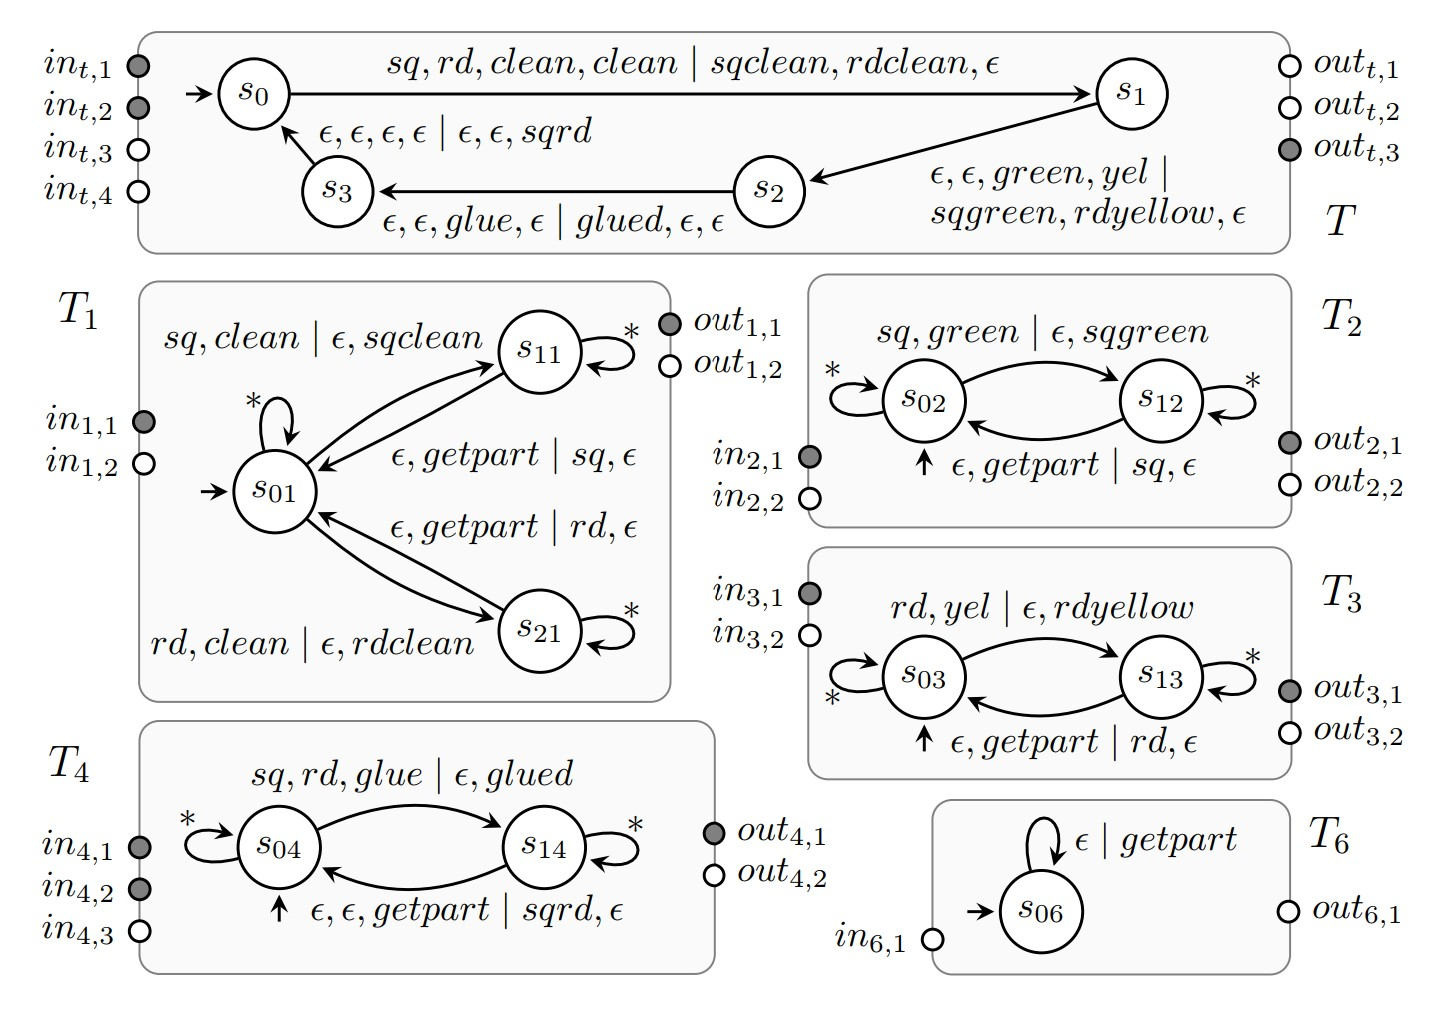
\includegraphics[scale=0.55]{images/milti-example.jpg}
\label{multi_example}
\caption{Target transducer T and resource transducers $T_{1}, . . . , T_{6}$ ($T_{5}$ is identical to $T_{1}$). Physical ports are shown greyed, and error states $s_{ej}$, are not shown. (\ast) on self-loops stands for $\epsilon, . . . , \epsilon, . . . | \epsilon, \epsilon$}
\end{figure}


\end{frame}

\end{document}
